\chapter{面向日常健康的面诊系统设计与实现}

通过对面诊系统的调研以及上一章节的用户研究,本文发现日常场景下的面诊技术的使用存在实用性、技术敏感性、文化敏感性等等问题,这里不再赘述。
针对这些问题,本文提出了对应的解决方案。同时,考虑到面诊技术发展迅速,目前的面诊系统设计都相对特异化,
本文希望提出一个相对统一的解决方案,提供标准的模型管理与接入方法,因此本文设计的面向日常健康管理的面诊系统需要着重解决以下几点问题:

\begin{itemize}
    \item 系统交互问题。
        \begin{enumerate}
            \item 日常场景下用户使用舌诊如何避免尴尬?
            \item 繁琐的使用流程影响长期使用。
            \item 专业术语带来的理解问题。
            \item 系统准确度带来的信赖问题。
            \item 诊断结果可视化带来的情绪问题。
        \end{enumerate}
    \item 技术敏感性问题。
        \begin{enumerate}
            \item 屏蔽移动设备间的差异性,降低设备要求。
            \item 系统稳定性问题。
            \item 模型管理与接入问题。
        \end{enumerate}
\end{itemize}

本章将从交互设计和系统设计方面阐述这些问题分别是如何解决的,其中设计策略实现部分着重解决系统交互问题,系统设计方面着重解决技术敏感性问题。


\section{设计策略实现1:日常可用性设计}
% 介绍原设计存在的缺点

% 在之前的研究中本文发现,目前的面诊交互设计在用户日常使用过程中存在以下问题:
\subsection{设计策略}
在之前的研究中本文发现,目前的面诊交互设计在用户日常使用过程中存在以下具体的可用性问题:
\begin{itemize}
    \item 日常场景下用户使用舌诊如何避免尴尬?
    与诊所环境不同,由于文化敏感性的问题,大部分中国人认为公共场合伸出舌头是非常不雅观的行为;部分用户也因为各种原因不愿意在非私人空间下拍自己的面部。这种设计对用户的日常使用产生了非常大的阻碍。
    \item 繁琐的使用流程影响长期使用。
    在用户持续使用的时候,用户每次诊断和上一次通常没有太大的变化。每次让用户重复相同的操作不仅非常费时,而且影响使用的积极性。
\end{itemize}

根据第三章增加日常可用性的思路,本文在设计实现过程中,邀请用户在日常使用的过程中参与迭代过程,最后实现了可用性设计原型。

\subsection{可用性设计实现}

\begin{figure}[h]
    \centering
    \subfigure[原型入口]{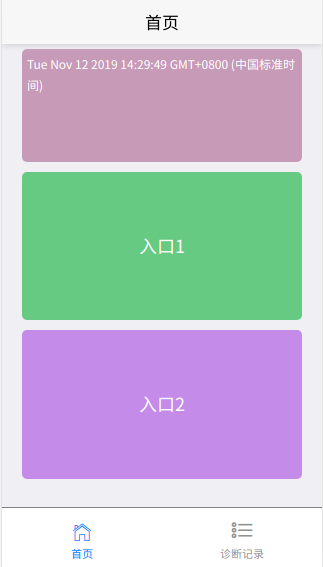
\includegraphics[width=4.5cm]{images/rukou.png}}
    \subfigure[新设计]{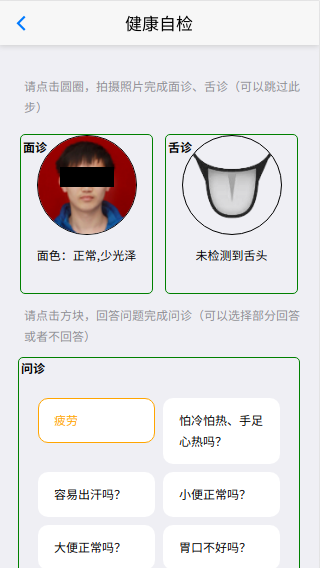
\includegraphics[width=4.5cm]{images/dialog1.png}}
    \subfigure[原设计]{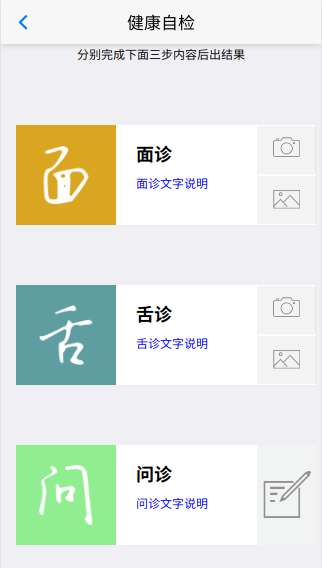
\includegraphics[width=4.5cm]{images/dialog2.png}}
    \caption{日常可用性验证实验}
    \label{fig:interface}
\end{figure}


在云中医应用中,用户在进行面部舌部拍照后,没有任何提示。具体的结果需要在用户一次回答13个问题之后,点击诊断才能知道面诊是否成功。
本文在面诊系统上,实现了一个用于对比的原型系统, 如图\ref{fig:interface} 所示。在该原型系统的首页,有两个入口,新设计和原设计分别对应本文的设计和云中医的设计,两个设计的功能相同。用户在进入实验原型系统的首页之后,可以自由选择入口,进入对应的界面完成诊断。
新设计和之前版本的云中医界面不同的是,诊断界面不仅提供了面诊舌诊问诊的入口,同时会将面诊舌诊的照片和中间结果直接显示在当前页面,用户能对于自己当前身体情况一个直观的感受。

\subsubsection{迭代过程}
\begin{figure}[h]
    \centering
    \subfigure[设计1]{
        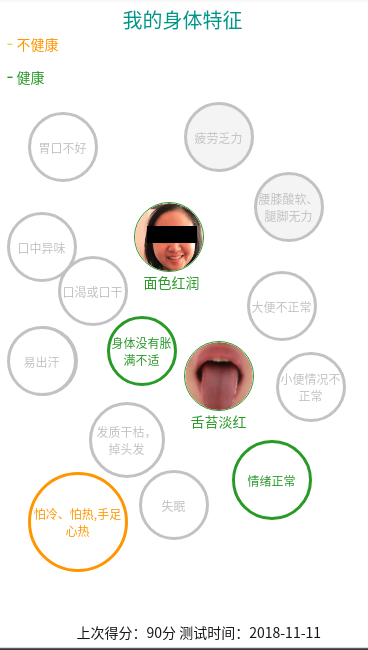
\includegraphics[width=3.5cm]{images/old1.png}
    }
    \subfigure[设计2]{
        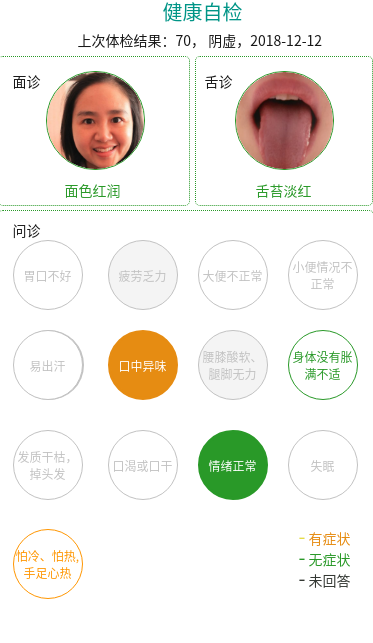
\includegraphics[width=3.5cm]{images/old2.png}
    }
    \subfigure[最终设计]{
        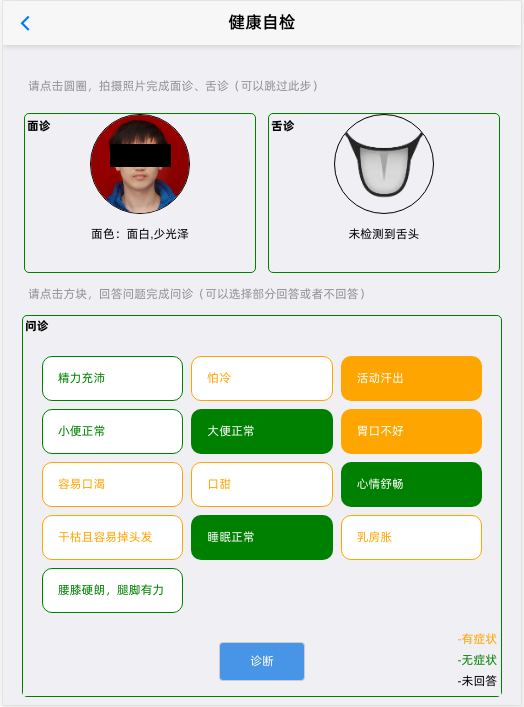
\includegraphics[width=4.5cm]{images/ui-1-1.png}
    }
    \caption{新设计迭代过程}
    \label{fig:diag_new}
\end{figure}
在进行可用性设计的过程中,原型系统经历了多次迭代。每次完成一版之后,我们会邀请小部分用户进行试用收集反馈并及时修改。
图\ref{fig:diag_new} 展示了部分中间的迭代版本和最终设计,其中设计1中的圆圈代表用户需要回答的问题,圆圈的大小代表影响的权重;
设计2简化了界面,统一了圆圈的大小;
最终设计进一步简化了界面元素,并把圆圈改为长方形,方便显示更多的提示信息。

\subsubsection{面诊问诊设计}

\begin{figure}[h]
    \centering
    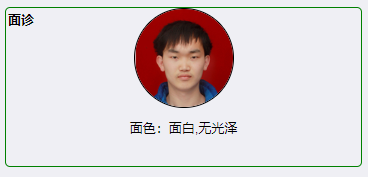
\includegraphics[]{images/diag_design.png}
    \caption{面诊元素设计}
    \label{fig:diag_design}
\end{figure}

根据日常可用性的设计策略,新设计简化了诊断的流程,面诊舌诊问诊在一个页面显示,并且所有的问题和操作都是可选的,不会出现必须要先面诊然后舌诊然后才能问诊的问题。其次,如图\ref{fig:diag_design}所示,新界面对面诊和舌诊进行了中间结果的反馈,面诊在用户拍照确认之后,会立即报告本次照片是否合格已经诊断的结果,用户不需要在点击诊断的时候才被提示照片不合格。

\subsubsection{问诊元素设计}
在问诊方面,新系统实现了最近一次记录保存,由于问题是可选回答的,所以用户只需要回答和自己上次的结果不一致的即可。

\begin{figure}[h]
    \centering
    \subfigure[上次回答有症状]{
        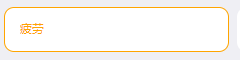
\includegraphics[width=6cm]{images/question/5.png}
    }
    \subfigure[上次回答无症状]{
        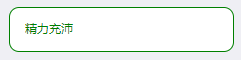
\includegraphics[width=6cm]{images/question/4.png}
    }
    \subfigure[本次回答有症状]{
        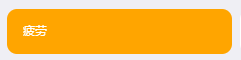
\includegraphics[width=6cm]{images/question/2.png}
    }
    \subfigure[本次回答无症状]{
        
\includegraphics[width=6cm]{images/question/3.png}
    }
    \subfigure[未回答]{
        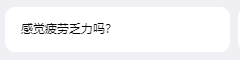
\includegraphics[width=6cm]{images/question/1.png}
    }
    \caption{问诊元素的状态}
    \label{fig:question_status}
\end{figure}

同时,如图\ref{fig:question_status}所示,本文对不同问题的回答结果进行了颜色的区分。有色实心代表本次回答,有色空心代表上次回答;橙色代表有症状,绿色代表回答的问题表现良好,没有症状;白色没有填充和边框,为黑字,代表未回答。实心颜色的代表的是用户本次有修改的问诊部分。

在方框内部的问题描述设计上,本文把默认的文字描述,显示为问题描述;一旦用户本次或者上次回答过该问题,则直接显示用户回答的结果。这样做的结果是,第二次用户点进来,就能看到上次的回答结果,这样能够对自己的身体情况有个快速的了解。

\section{设计策略实现2:系统可解释性设计}

\subsection{设计策略}

根据之前的用户研究的结果来看,当前系统存在以下问题:

\begin{itemize}
    \item 专业术语带来的理解问题。
    由于当前诊断和打分模型存在改进的空间,部分的用户对结果产生了怀疑或者对结果不理解的问题。同时,日常健康场景下,没有专业医护人员的帮助,普通用户由于缺乏对应的专业知识,对应用的理解还有很大的提升空间。
    \item 系统准确度带来的信赖问题。
    在面诊系统由权威的诊所迁移到日常场景后,许多用户对系统的结果持怀疑态度,从而导致他们不信赖系统。在没有其他的评估机制验证结果有效性的前提下,也会让用户对系统产生怀疑。
    \item 诊断结果可视化带来的情绪问题。
    直白地展示诊断结果,特别是系统给出负面结果时,会让用户产生明显的消极情绪并放弃继续使用。
\end{itemize}


目前主要对提高用户对系统理解程度的方式一般是通过文字、可交互式元素或者可视化的方法描述来暴露算法置信度、暴露中间结果、提供当前数据和原始数据对比等实现\cite{wang2019designing, kocielnik2019will},
其中文字化的描述适合对系统的背景、或者专业名词进行解释;暴露算法的中间结果以及置信度,能激起用户探索算法原理的好奇心以及提高对结果的容忍程度。
此外,具有自解释的模型如卷积神经网络,attention机制等也是当前研究的热点。

但是,考虑到涉及医疗数据的敏感性,暴露原始数据的方式并不适合在面诊系统中使用。
模型的自解释性并不是当前众多面诊算法的通用属性,本文考虑的是日常场景下通用的面诊系统实现,而不是通过强依赖特定模型来实现系统的可解释性。
考虑到一次面诊过程涉及到诸多子过程,最终本文希望通过对诊断过程进行拆分,将模型的诊断过程对用户可见,并使用合适的文字和可交互元素对结果进行解释,来提高用户的交互体验。


不过面诊系统在日常生活中的应用是一个全新的场景,需要解释的对象是什么,通过何种交互元素进行解释,具体细节如何实现仍是未知的问题。


\subsection{可解释设计实现}

在第四章中本文详细介绍了目前技术探针中可用的模型,根据本文系统和模型的特点,解释在呈现的时候,实现的解释方法大致可以分为以下几种:

\begin{enumerate}
%  为什么要解释,文字解释的作用。
    \item 如图\ref{fig:face_diags}所示,结果中文字结果有提示、可以进行点击。如果用户点击了健康报告的分数,会通过弹窗通过文字描述进行详细的解释。

    \item 如图\ref{fig:question_weight}所示,通过雷达图的可视化方式直接显示对结果的影响,交互性比较强。 
    
    \item 如图\ref{fig:report_expalin_score}所示,通过可交互元素折叠列表对不同条件下的计算公式进行解释。
\end{enumerate}

用户在使用系统的过程中,需要经过面诊、舌诊、问诊等流程,最终得到诊断的结果。为本文根据交互研究中用户反馈的问题,对用户完成一次诊断的中间流程以及最终的结果都进行了解释。

\subsubsection{面诊舌诊的解释}

\begin{figure}[htbp]   
    \centering
    \subfigure[不解释]{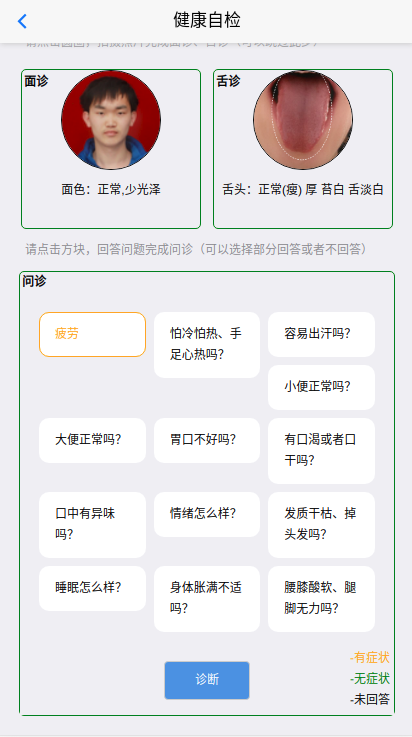
\includegraphics[width=4.5cm]{images/face_tongue.png}}
    \subfigure[解释]{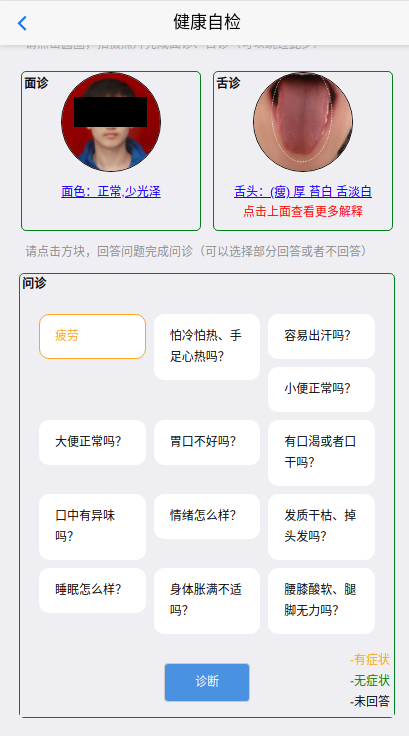
\includegraphics[width=4.5cm]{images/exp_face_tongue.png}}
    \subfigure[详细解释]{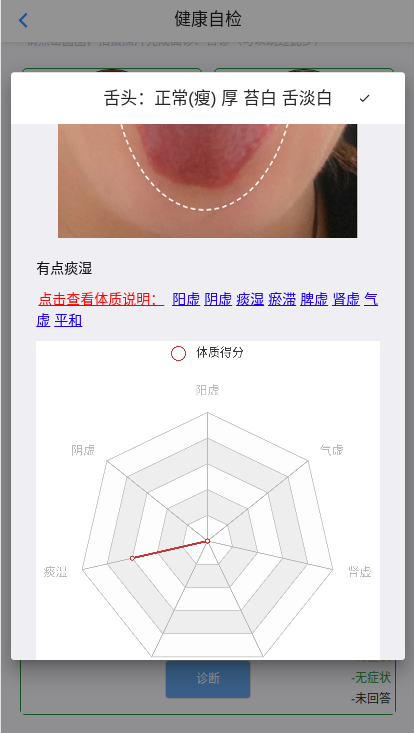
\includegraphics[width=4.5cm]{images/exp_tongue.png}}
    \caption{面诊舌诊的解释}
    \label{fig:face_diags}
\end{figure}

面诊和舌诊流程比较类似,都是通过分析面部或者舌部图片,得到分析结果,因此这两部分合并放到一起解释。
面诊和舌诊断添加解释主要体现在结果的解释,包括中间结果和对各种体质倾向的影响。
用户查看解释之后,能够大致了解本次拍照是否成功,并且知道目前面诊的结果,以及可能会对最终的健康报告造成哪些影响。具体如图 \ref{fig:face_diags} 所示:

(a) 没有解释的设计,只能看到结果。

(b) 有解释的设计,通过点击面诊或者舌诊结果,查看对结果的解释。

(c) 点开解释之后,系统会弹窗进行详细的解释,不仅可以看到当面诊断的中间结果,也能看到这次诊断的体质倾向得分。

接下来介绍该原型中各个解释的细节具体如何实现。


\subsubsection{问诊的解释}

\begin{figure}[htbp]
    \centering
    \subfigure[不解释]{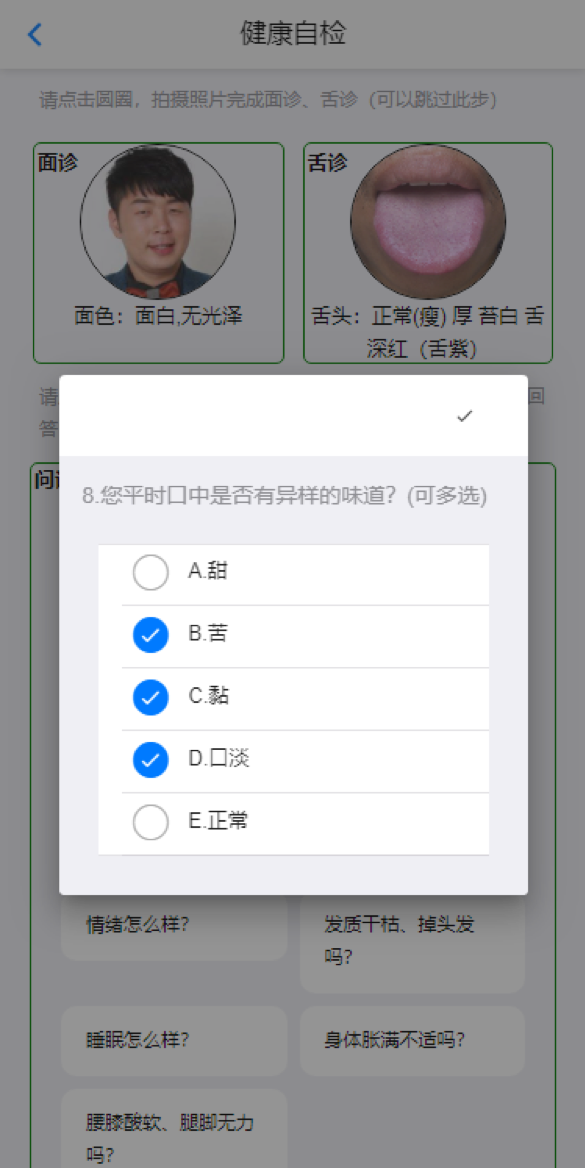
\includegraphics[width=5cm]{images/questions.png}}
    \subfigure[解释体质术语]{
        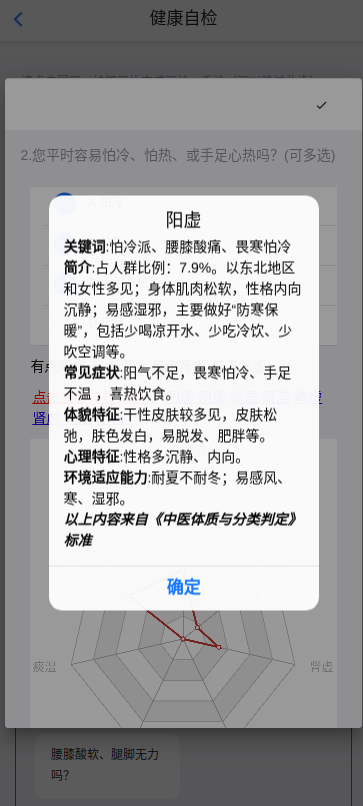
\includegraphics[width=5cm]{images/exp_phy.png}
    }
    \caption{问诊的解释}
    \label{fig:questions}
\end{figure}

问诊的过程中解释的主要实现,是通过对体质的专业术语和每个答案对结果的影响进行解释,具体实现如图 \ref{fig:questions} 所示:

(a) 不解释的设计,用户回答问诊问题之后,没有任何提示或者解释。

(b) 有解释的设计,用户在进行问诊过程中,可以立即看到每个答案对结果的影响,通过下方的雷达图显示了影响的体质倾向类型和具体的数值。
雷达图的更新是实时根据用户的选择进行更新的,用户可以通过点击不同的选项查看不同选项对应的雷达图。

(c) 点开体质的解释之后,会通过弹框的方式,对中医术语中,各种体质的解释。对于体质内容的解释文字引用自 《中医体质分类研究》标准。


\subsubsection{诊断结果的解释}
\begin{figure}[htbp]
    \centering
    \subfigure[不解释]{
        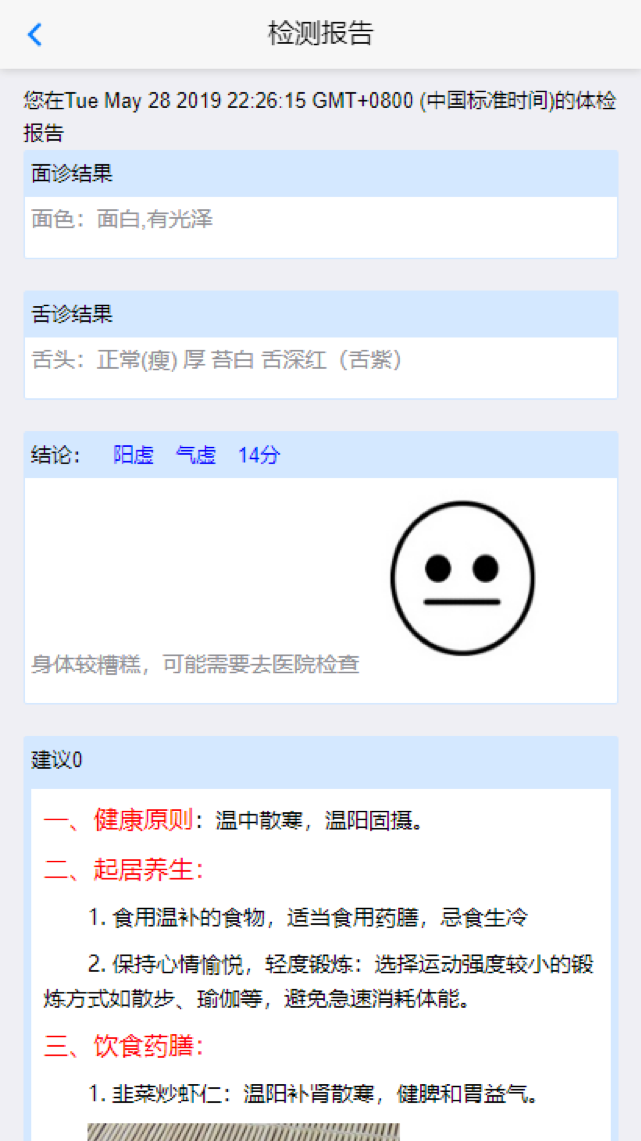
\includegraphics[width=4.5cm]{images/report.png}
    }
    \subfigure[解释]{
        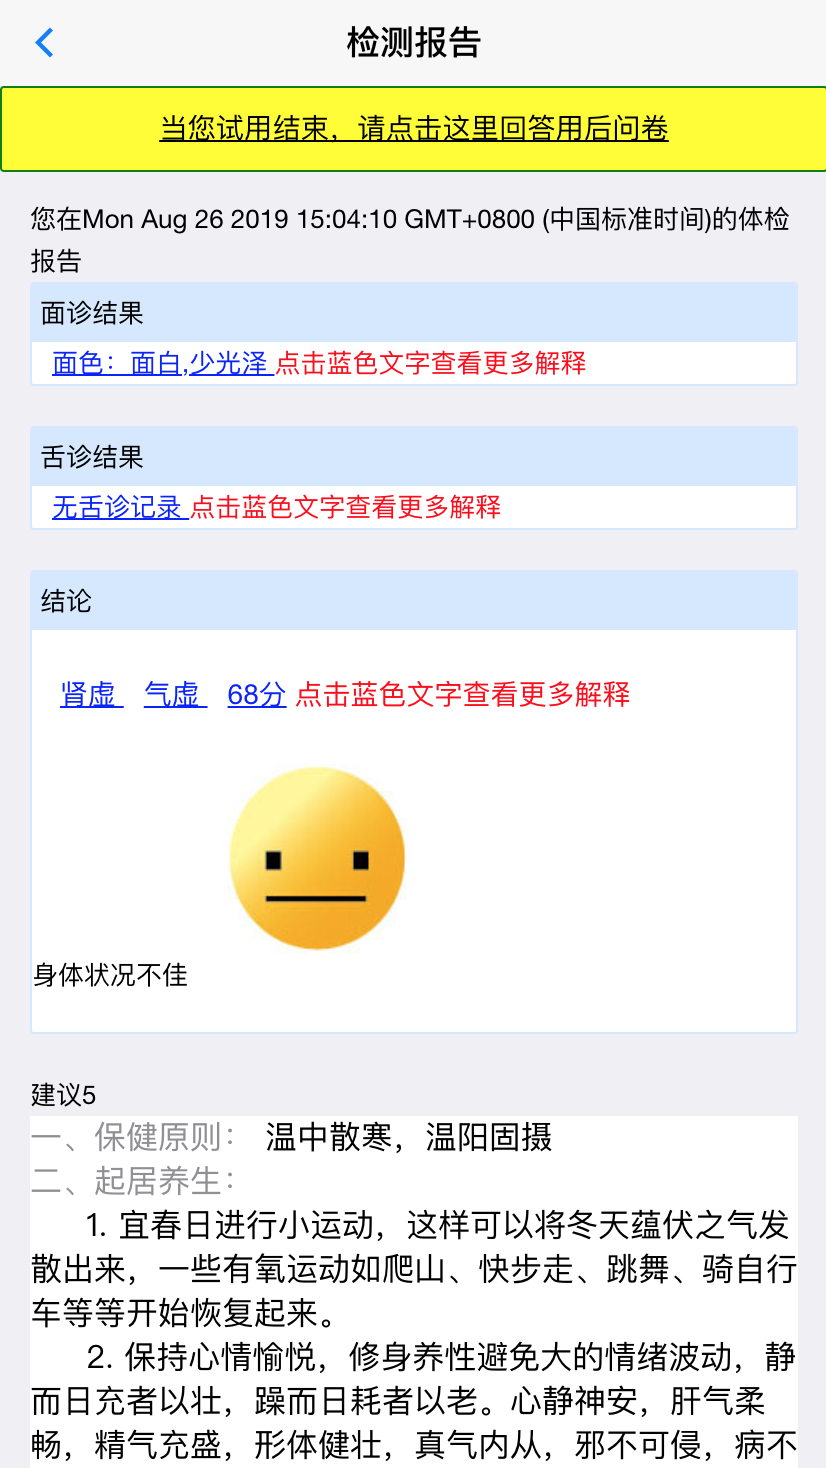
\includegraphics[width=4.5cm]{images/report3.png}
    }
    \caption{诊断结果的解释}
    \label{fig:exp_result}
\end{figure}

诊断结果的解释主要是对结果的判断依据和相关原理进行解释,具体如 \ref{fig:exp_result} 所示:

(a) 在没有解释的设计中,用户在诊断结果页面,可以看到自己的健康分数和体质结果,并且会在后面给出对应的养生建议和实践,但是给出的结果是不可点击的;

(b) 在有解释的设计中,用户可以点击诊断结果,包括面诊结果、舌诊结果,体质、健康分数。用户点击之后,可以通过之后的弹框,看到详细的解释,如点击健康分数之后,可以了解这个分数是根据哪些指标,通过哪一个算法计算过来的。

从\ref{fig:exp_result} 中可以看出有解释的设计中,用户点击结果后,会通过弹框解释结果。可以点击查看的结果的解释有:面诊舌诊结果的解释,健康分数的解释,体质的解释,接下来分别介绍如何实现。



\subsubsection{健康分数的解释}
问诊结果的解释主要是对用户解释诊断结果是如何计算,以及那些问诊的问题对结果有影响,影响程度多少。

\begin{figure}[htbp]
    \centering
    \subfigure[相关问题]{
        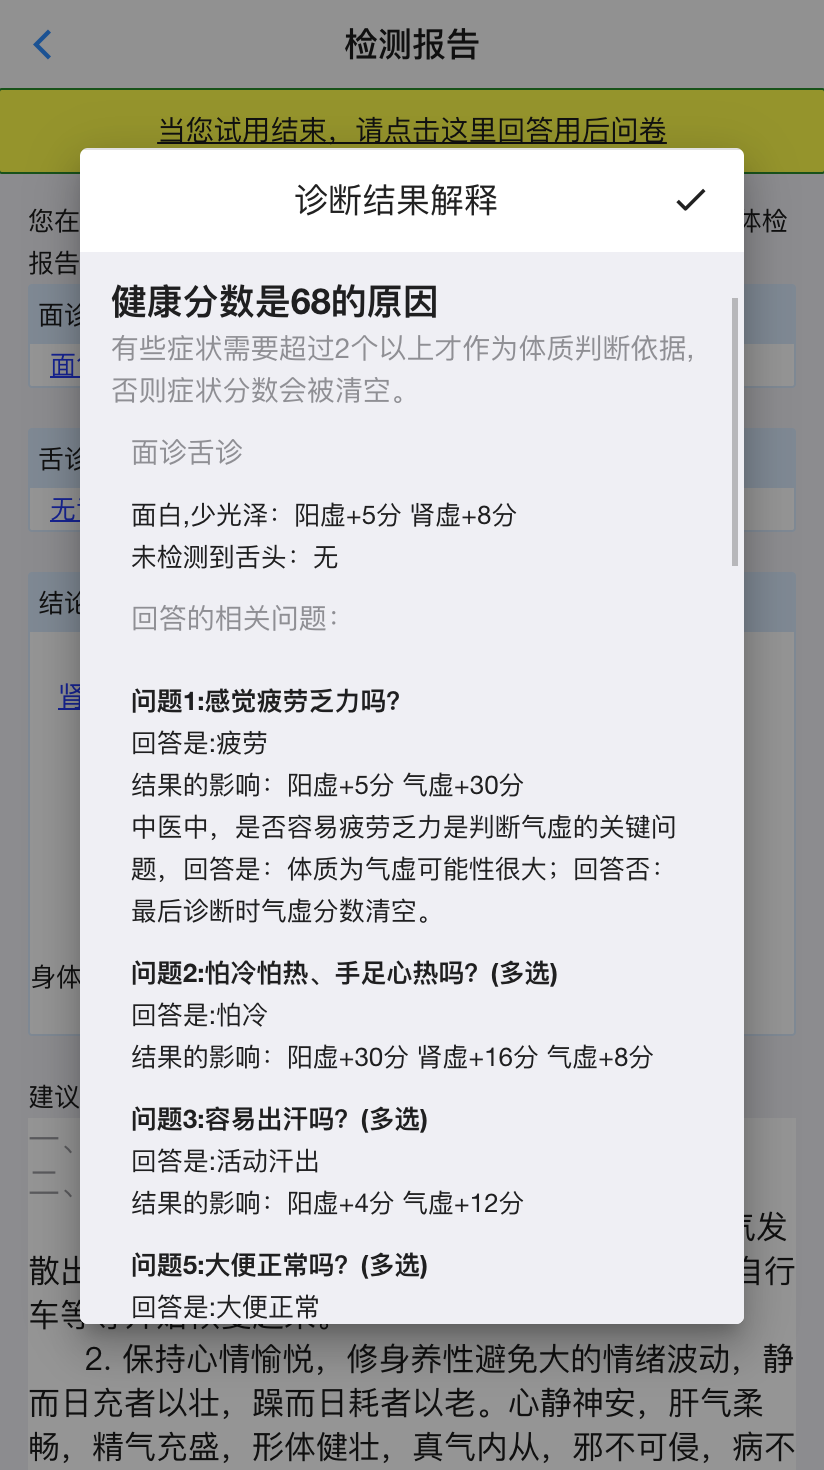
\includegraphics[width=4.5cm]{images/report7.png}
    }
    \subfigure[雷达图]{
        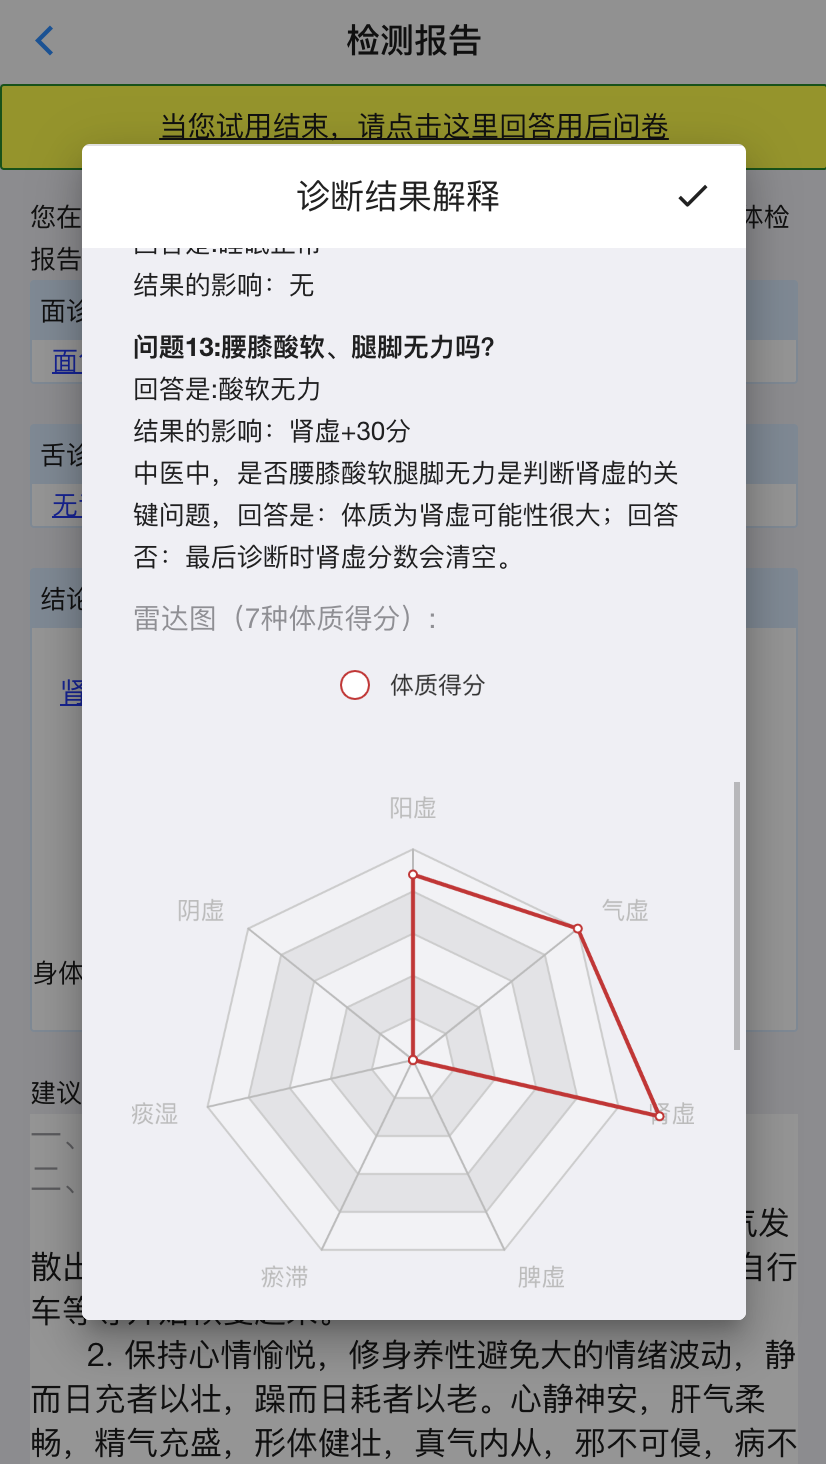
\includegraphics[width=4.5cm]{images/report8.png}
    }
    \subfigure[计算公式]{
        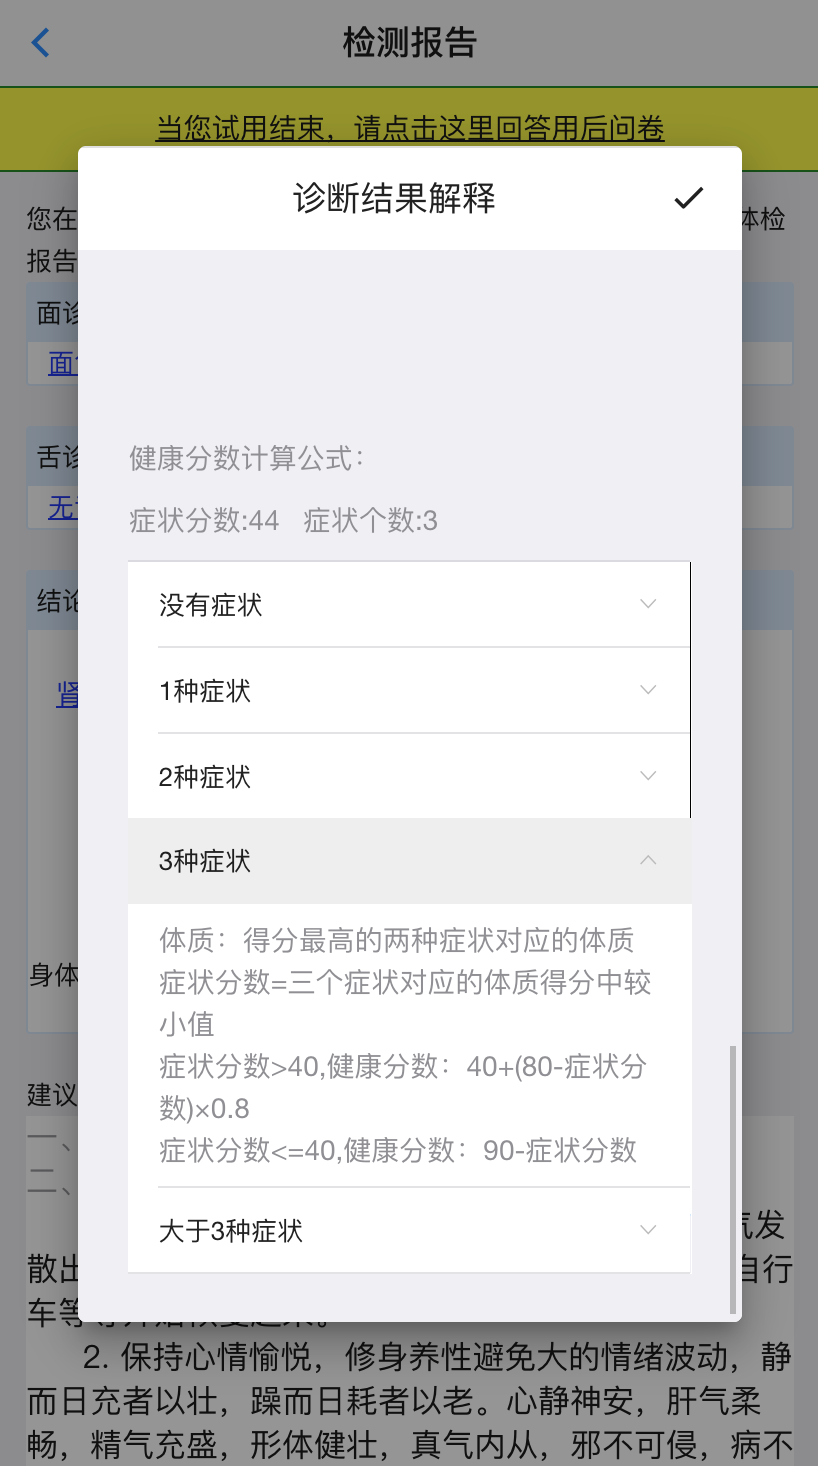
\includegraphics[width=4.5cm]{images/report9.png}
    }
    \caption{健康分数的解释}
    \label{fig:report_expalin_score}
\end{figure}

如图\ref{fig:report_expalin_score}所示,用户点击诊断页面的分数之后,弹窗里会显示分数相关的问题、雷达图和分数计算公式。

分数相关问题,展示了面诊舌诊对体质分数的影响和问诊对体质分数的影响,无影响的问题则不会显示。

用户每次回答一个问诊的问题,或者进行面诊舌诊断,都会对体质的倾向分数产生一定的影响。在规则系统中,体质倾向分数的变化分两种,一个是分数的累加,另一种是体质倾向分数的清空。

雷达图对体质分数进行了汇总,给用户展示最终个人的体质倾向的结果。

根据规则系统,解释页面的计算公式一共有5种类别。用户具体属于哪个类别,使用哪一套计算公式,是由用户当前的症状的个数来决定的。

本文使用选项卡的方式,将所有的打分计算公式全部暴露给用户,并且默认打开当前计算公式的选项卡。


\section{系统设计}

本小节将介绍本文如何在系统设计层面解决本文在上一章发现的技术敏感性问题以及为可解释性设计提供基础:

\begin{enumerate}
    \item 屏蔽移动设备间的差异性,降低设备要求。
    \item 系统稳定性问题。
    \item 模型管理与接入问题。
\end{enumerate}


\subsection{诊断任务建模}
本文在实现一个诊断系统之前,对系统流程进行了建模。
诊断任务建模是诊断任务拆解的基础,通过对诊断任务拆解,可以将诊断过程的中间结果暴露出来,方便后续实现可解释性设计。

从用户输入,到得到最终的结果,将会并发地、顺序地调用各类模型资源。因此,本文将整个过程定义成一个多输入节点,单输出节点的有向无环图。

对于其中的每一个节点,本文给出的定义如下:

\begin{lstlisting}[language={Python}, title=model.py]
class BaseModel(model):
    input_json = ''
    output_json = ''
    type = 0
    next_models = None
    status = 0
    
\end{lstlisting}

其中输入和输出以json的方式记录,type用于记录模型的类型,next models 用于指定节点的下游,status表示节点状态。

\begin{figure}
    \centering
    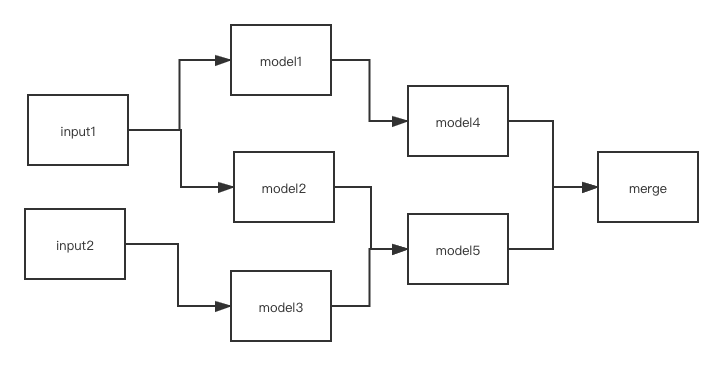
\includegraphics[width=15cm]{images/model_dag.png}
    \caption{模型调用有向无环图}
    \label{fig:model_dag}
\end{figure}

如\ref{fig:model_dag}所示,整个诊断任务由一个有向无环图组成,每个节点都是一个对应的独立服务。

整个有向无环图有两个特殊的节点,分别是input节点与merge节点。

\begin{itemize}
    \item input节点
\end{itemize}

input节点用于保存用户的原始输入信息,同时触发有向无环图开始执行。
用户在使用面诊系统的过程中,通常都是一步一步地传入自己信息。
多个input节点的设计,可以在用户面诊的过程中,动态地执行图中的部分节点,而不是要等待所有输入完成之后再执行。
此外,input节点还负责用户输入的处理,用于兼容不同输入设备的输入,理论上可以兼容各类不同的硬件输入设备。

\begin{itemize}
    \item merge节点
\end{itemize}

merge节点用于采集上游节点的输出,并将结果进行合并。
merge节点可以兼容多输出的场景,在系统需要多个输出的时候,可以把输出节点的叶子节点加上merge节点,merge节点负责将这些结果汇总。

模型间的顺序与并发执行,都由该有向无环图定义,后续增加删除模型也非常方便。
同时,节点拆分的设计,可以实现节点级的缓存,提高系统的效率。


\subsection{系统模块设计}
为了适应各种类型的面诊算法和交互设计,客户端版本更新的速度会非常快,同时本文希望用户的设备类型不能成为障碍,跨平台是较好的解决方法。


如图\ref{fig:system}所示,系统整体运行在容器环境下,使用Redis和MySQL作为持久化工具,主要分为三部分:服务端和客户端,算法模型通过容器的方式(docker\footnote{https://www.docker.com/}、kubernetes\footnote{https://kubernetes.io/})服务化成模型池。
\begin{figure}
    \centering
    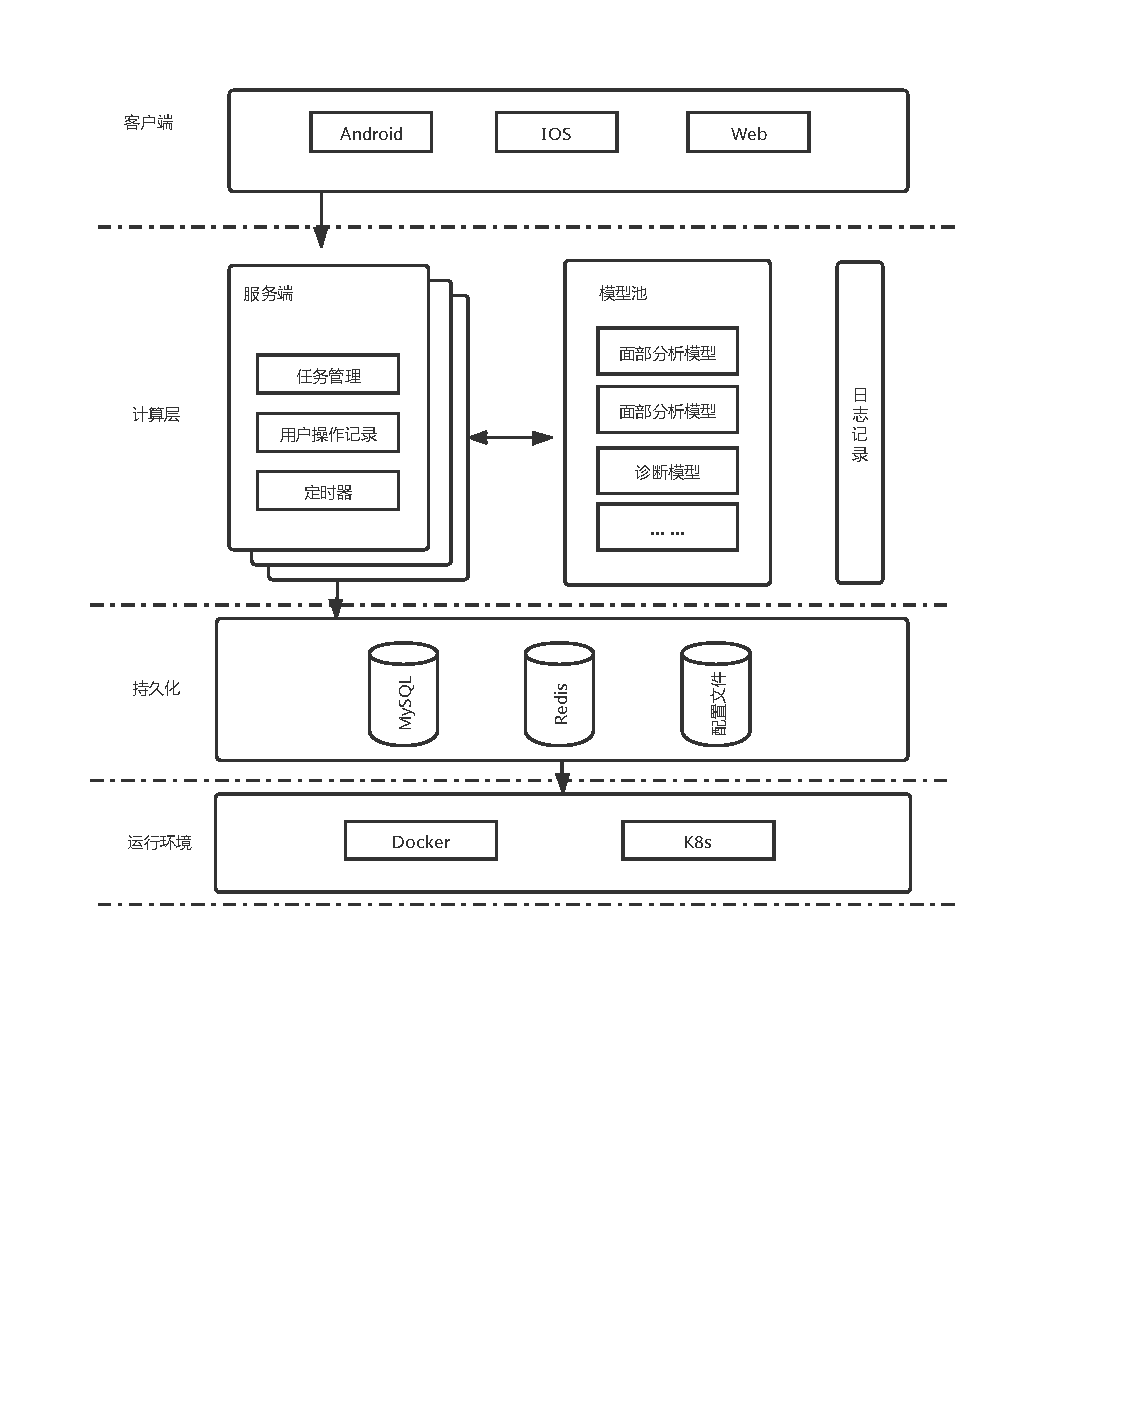
\includegraphics[width=15cm]{images/system2.pdf}
    \caption{诊断系统设计}
    \label{fig:system}
\end{figure}
客户端包括Android、IOS和Web平台的客户端,与用户交互密切相关,负责用户面诊的流程已经数据上传,通过请求服务端的接口完成面诊和记录用户的操作信息;
服务端通过调用模型池的相关服务,为客户端提供接口服务。
模型池是指在容器环境下通过容器服务化的方式下所有可用的模型服务的统称,为服务端提供计算服务,完成面部图片分析,舌部图片分析等任务。
大多数模型格式为二进制可执行文件或者本地模型文件的形式,为了方便服务端调用,需要对其进行服务化。

服务化指的就是将算法模型,打包成可调用的服务。其中本文的模型服务化通过Flask框架实现,每一个模型的服务都可以对应服务端中的一个计算任务。
服务端在任务管理模块中定义了任务的输入输出格式,模型池中的服务只要保持格式一致就可以保证服务端能够顺利调用对应的模型服务。

一次诊断的大致流程如下:用户通过客户端,上传图片或者回答问题,客户端则向服务端发起请求。
服务端收到请求之后,进行任务分配,对分配到任务的服务端实例,调用模型池中对应的模型完成特征提取或诊断打分,同时将数据持久化到mysql和硬盘中,然后把结果返回给客户端。
客户端收到服务端的结果后,进行结果的展示。

\section{模型池}
% 什么是模型池
本文提出一个模型池的概念将面诊模型与服务端解耦,方便以后更新模型。模型池由多个独立可用的模型服务构成,每个服务对应模型调用有向无环图的一个节点,节点和节点之间通过http接口调用完成和服务端的交互进行任务处理。

% 为什么要模型池
提出模型池的概念,是为了将模型和服务端独立,方便以后添加或删除模型,同时使系统不局限于当面的诊断模型,方便系统拓展到其他交互研究领域。
此外,将模型独立做成服务,可以动态增加模型运行的实例个数,提高计算能力和稳定性。


% \begin{figure}[h]
%     \centering
%     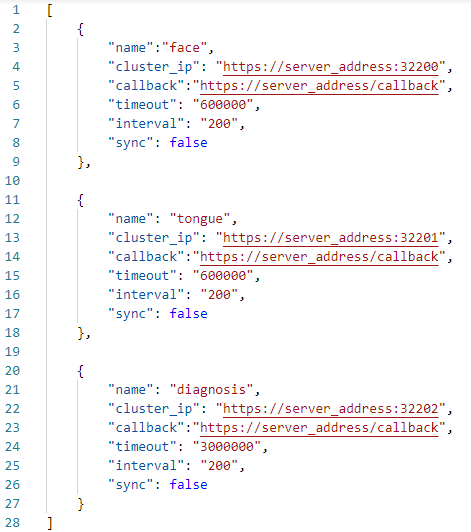
\includegraphics[width=15cm]{images/services2.png}
%     \caption{模型池配置}
%     \label{fig:services}
% \end{figure}

\begin{lstlisting}[language={Python}, title=services.json]
[
{
    "name":"face",
    "cluster_ip": "https://server_address:32200",
    "callback":"https://server_address/callback",
    "timeout": "600000",
    "interval": "200",
    "sync": false
}, 

{
    "name": "tongue",
    "cluster_ip": "https://server_address:32201",
    "callback":"https://server_address/callback",
    "timeout": "600000",
    "interval": "200",
    "sync": false
},
...
]
    
\end{lstlisting}

% 如何实现的
如services.json所示,模型池保存一个<模型类型, cluster ip> 的映射,记录可用的模型和调用地址, cluster ip是由k8s(kubernetes)提供的集群调用地址。记录通过json文件的格式,记录在本地文件中。
其中sync参数代表是否同步返回结果,如果设置成异步返回,则通过调用callback地址将结果回调给服务端,服务端收到回调之后保存结果。
timeout字段用于预先设置服务的超时时间,由于不同的服务计算时间不同,可以根据模型的实际运行速度进行调整。
interval字段表示失败或者超时的重试间隔,默认设置为200毫秒。

服务的稳定性和高可用需要做到服务之间相互独立和多实例同时运行,docker和k8s是容器化解决方案和容器编排工具,能够很方便地实现这个需求。
模型服务使用docker进行打包,通过k8s管理多个模型高实现可用。
服务端通过k8s提供的cluster ip进行调用,这样能保证在大量用户同时请求模型服务时,某个模型服务如果出错,集群中的其他模型服务能够响应请求。


\subsection{模型服务化}
为了方便模型管理,本文将模型和客户端服务端独立出来,打包成独立可运行的服务。

\subsubsection{具体实现}
Flask\footnote{https://palletsprojects.com/p/flask/}是一个基于Python语言的轻量级Web框架,开发者通过极少的代码可以快速实现一个Http服务。服务化的过程是通过Flask框架建立一个Http的服务,把特征提取模型打包成服务。

本系统对模型的接入标准如下:每个模型池中的服务,接受http的请求,对传过来的数据进行计算。每个请求通过路由规则找到需要请求的模型服务。模型服务service根据模型计算能力的不同,需要具体独立实现。在实现service的时候,为了减少服务之间读写的竞争,模型池中的服务只进行计算,不进行对mysql和redis的读写,结果的持久化由服务端完成。service的内部逻辑需要把服务设计成无状态:如果模型计算需要创建临时文件,计算结束需要删除临时文件。使用json作为通讯格式,方便模型服务与系统快速接入。

\subsection{现有模型概况}
基于在云中医技术探针工作的基础上,目前现有两类已拆分的模型,特征提取模型(面部和舌部两种)和诊断打分模型,分别有对图片进行特征提取和对特征进行打分的能力。
特征提取模型对用户输入的特征(面部或者舌部图片)进行特征提取,而诊断打分模型,由一系列规则组成,定义了每一个特征对最终的打分输出影响的规则。

\begin{figure}[ht]
    \centering
    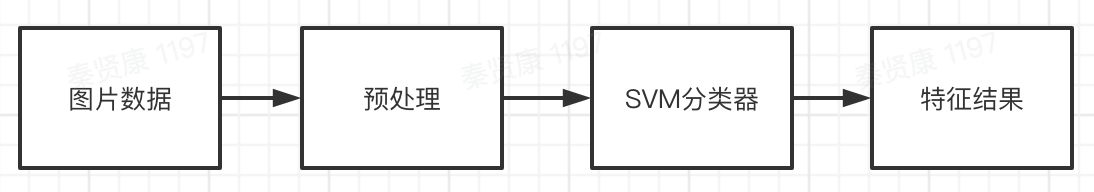
\includegraphics[width=15cm]{images/model.png}
    \caption{特诊提取模型}
    \label{fig:my_model}
\end{figure}
目前用到的模型,基于opencv和其自带的svm,使用c++实现了图片特征的提取和分类。
如图\ref{fig:my_model}所示,在云中医的端到端模型中,用户面部和舌部数据会经过预处理,如使用高斯混合模型\cite{Hu2016Robust} 进行ROI区域提取(提取舌部,唇部,面部区域等),
然后由svm分类器,判断该样本中是否包含嘴唇、嘴唇的特征等。
在每个模型的基础上,最后由一个诊断规则根据每个模型的输出,得到最终的诊断结果。
svm分类器的训练数据来自各个医院的临床真实数据。

\begin{figure}[ht]
    \centering
    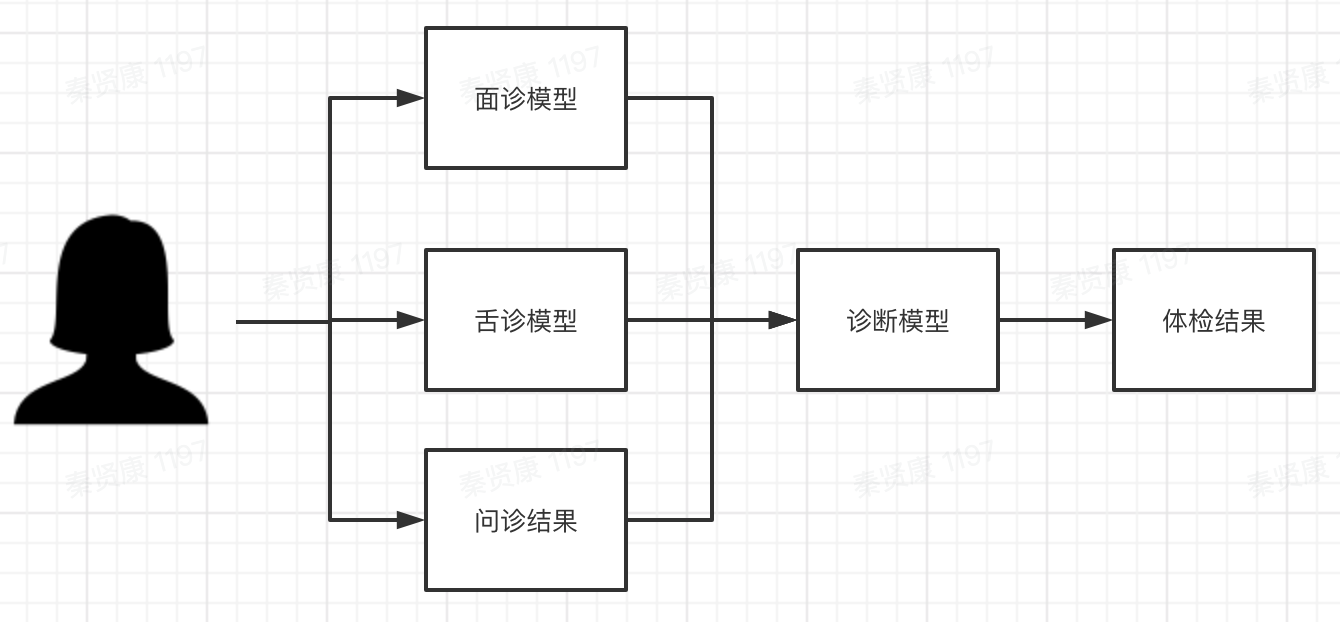
\includegraphics[width=15cm]{images/model2.png}
    \caption{诊断模型}
    \label{fig:my_model2}
\end{figure}
诊断规则由上海中医药大学和专业的医生编写,规则的表现形式:把人的体质分为7大体质倾向(阳虚,阴虚,痰湿,瘀滞,脾虚,肾虚,气虚),根据用户的特征,修正体质倾向的数值,最后得到最终的体质和健康得分。
在后续随机抽取患者的对比实验中,准确率达到了90\%以上 \cite{Zhang2018Study}。

本文涉及的算法的具体实现不多做介绍,详细细节可见\cite{Zhang2018Study, Qiu2015Adaptive, Hu2016Robust},接下来只介绍拆分后的模型的输入输出的功能,模型的计算能力如表\ref{tab:face-feature}, 表\ref{tab:tongue-feature},表\ref{tab:diag-feature}所示。
\subsection{脸部特征提取模型}

\begin{table}[h]
    \centering
    \begin{tabular}{lll}
        \toprule
        特征          & 特征描述     & 特征内容 \\ 
        \midrule
        faceDetectRes & 人脸   & 0:未检测出人脸,1:成功检测出人脸  \\
        faceColor     & 面部颜色 & 0:面白,1:面黑,2:面红,3:面黄,4:面青,5:正常 \\
        faceGloss     & 面部光泽 & 0:有光泽,1:少光泽,2:无光泽\\
        lipDetectRes  & 嘴唇   & 0:未检测出嘴唇,1:成功检测出嘴唇\\
        lipColor      & 嘴唇颜色 & 0:淡白,1:淡红,2:红,3:暗红,4:紫   \\
        \bottomrule
    \end{tabular}
    \caption{脸部特征提取模型输出}
    \label{tab:face-feature}
\end{table}

如表 \ref{tab:face-feature} 所示,脸部特征提取模型,输入为面部特征图片,输出有以下几个维度:

\begin{enumerate}
    \item 是否检测到人脸(faceDetectRes):如果没有检测到人脸,则剩余所有维度无效,且取值为0。

    \item 是否检测到嘴唇(lipDetectRes): 如果没有检测到嘴唇,嘴唇颜色的结果无效且取值必定为0。

    \item 面部颜色、面部光泽(faceColor、faceGloss) : 面色和光泽是对预处理之后的图片,去除眼口鼻区域的图片进行面色和光泽信息提取的结果。

    \item 嘴唇颜色(lipColor): 嘴唇颜色的结果从浅到深分别为淡白,淡红,红,暗红,紫。
\end{enumerate}


\subsection{舌部特征提取模型}

\begin{table}[h]
    \centering
    \begin{tabular}{lll}
        \toprule
        特征 & 特征描述 & 特征内容 \\ 
        \midrule
        tongueDetectRes & 舌体 & 0:未检测出舌像,1:成功检测出舌像 \\
        tongueCrack & 舌裂纹 & 0:未检测到裂纹,1:成功检测到裂纹 \\ 
        tongueFatThin & 舌胖瘦 & 0:正常(瘦),1:胖舌 \\
        tongueCoatThickness & 舌苔厚薄 & 0:薄,1:厚 \\
        tongueCoatColor & 舌苔颜色 & 0:苔白,1:苔黄 \\
        tongueNatureColor & 舌质颜色 & 0:舌暗红,1:舌淡白,2:舌淡红,3:舌红,4:舌紫\\
        \bottomrule
    \end{tabular}

    \caption{舌部特征提取模型输出}
    \label{tab:tongue-feature}
\end{table}

如表 \ref{tab:tongue-feature} 所示,舌部特征提取模型,输入为舌头图片,输入有以下几个维度:

\begin{enumerate}
    \item 是否检测到舌体(tongueDetectRes): 如果没有检测到舌体,则剩余所有维度无效,且取值为0。

    \item 是否检测到舌裂纹(tongueCrack): 舌裂纹是最终特征,剩余特征是否有效和该标志位没有关系。

    \item 舌头特征(tongueFatThin、tongueCoatThickness、tongueCoatColor、tongueNatureColor): 包括舌胖瘦,舌苔的厚薄,颜色和舌质颜色。

\end{enumerate}

\subsection{诊断模型}

\begin{table}[h]
    \begin{center}
        \begin{tabular}{lll}
            \toprule
            特征 & 特征描述 & 特征内容 \\ 
            \midrule
            healthScore & 健康分数 & 0-100 \\
            healthType & 是否包含某种体质 & {[}0, 0, 0, 0, 0, 0, 0{]} \\ 
            questionScore & 各种问题的体质得分 & {[}0, 0, 0, 0, 0, 0, 0{]} \\
            symCount & 各种体质症状个数 & {[}0, 0, 0, 0, 0, 0, 0{]} \\
            symNum & 总体体质症状个数 & 0-13 \\
            baseScore & 基本分数 & 0-100 \\
            phy & 体质结果 & 八种体质中的一种\\
            \bottomrule
        \end{tabular}
    \end{center}
    \caption{诊断打分模型输出}
    \label{tab:diag-feature}
\end{table}

% 原版的云中医应用中,只给用户暴露了健康分数和体质结果。

如表 \ref{tab:diag-feature} 所示,最终诊断打分模型的体质结果输出为阳虚、阴虚、痰湿、瘀滞、脾虚肾虚、气虚、健康中的一种,具体的特征说明如下:
\begin{enumerate}
    \item 健康分数(healthScore): 打分的最终健康分数,由baseScore、symsNum、questionScore计算而来。

    \item 体质类型(healthType): 大小为7的数组,对应阳虚、阴虚、痰湿、瘀滞、脾虚肾虚、气虚、健康。如果包含某个体质,对应位置的值为1。

    \item 问题得分(questionScore): 一共有13个问题,每个问题都会影响最终体质的倾向得分, questionScore是所有问题的得分的累加。

    \item 症状个数(symCount): 13个问诊问题中,对应有某个体质特征的症状的累加。

    \item 总体症状个数(symNum): symCount的求和。

    \item 基本分数(baseScore): 诊断任务中,healthScore = baseScore*p + 症状分数*q ,对应不同的症状个数,计算最终得分用的baseScore是不一样的。 
p和q是模型中预设的权重, 症状分数由问题得分计算而来。

    \item 体质结果(phy): 和healthType对应,给出用户的体质倾向。
\end{enumerate}

诊断打分模型的最终输出是健康分数(baseScore)和体质结果(phy),其他的特征输出,是为了后续的算法可解释性做准备。同时,模型的特点也影响了本文最终实现可解释设计的实现方案。


\section{服务端}

服务端使用Python实现,允许有多个服务端实例同时运行,共同处理用户发起的诊断任务,使用redis和mysql进行数据的持久化。
% Redis \footnote{https://redis.io/}是基于内存的分布式数据库,在本系统中主要保存服务端可用节点的信息。
% Mysql \footnote{https://www.mysql.com/} 是当前比较流行一个关系型的数据库,在本系统主要主要保存用户操作信息,任务信息等。       

服务端的主要模块如图 \ref{fig:server} 所示,其中用户操作记录管理提供了网页端的管理界面,能够在线地对用户操作进行查询导出;任务管理为客户端提供了任务提交和结果查询接口,为客户端的面诊、舌诊、问诊提供支持。

系统通过设置定时器,定期地发送心跳包进行主从竞选,主节点会进行任务分配,主节点和从节点则对分配到的任务进行执行,调用模型池中对应的模型服务完成任务。


\begin{figure}[ht]
    \centering
    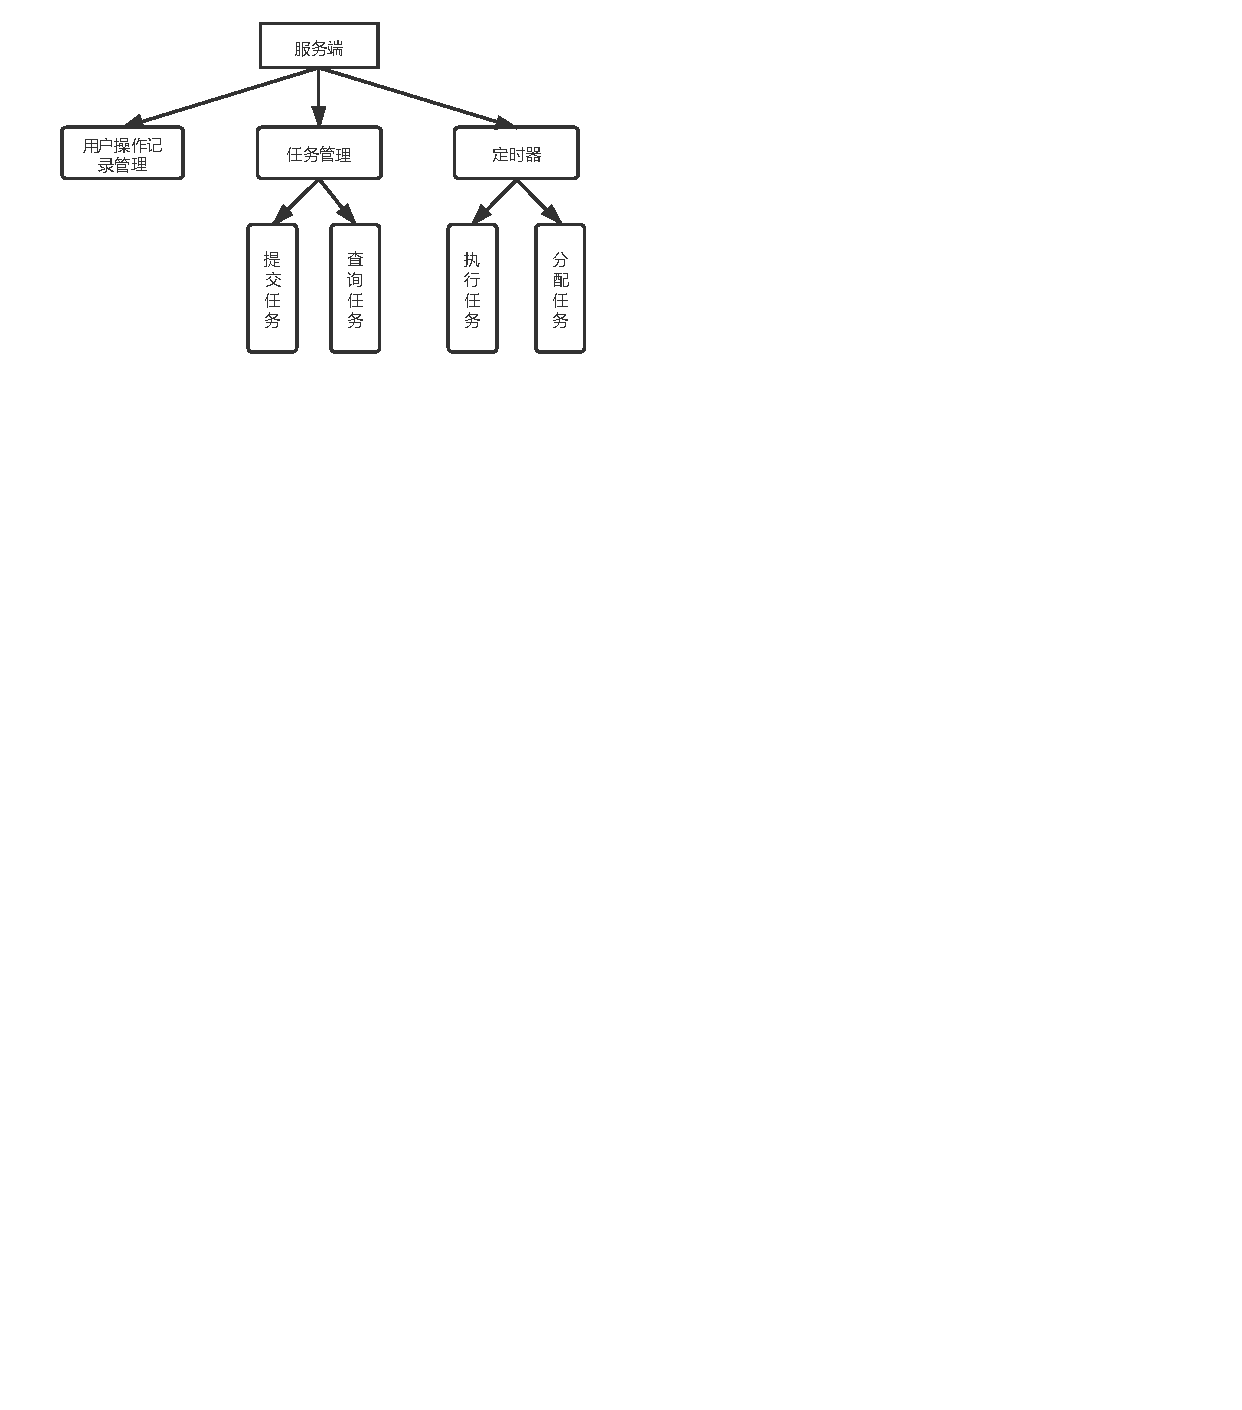
\includegraphics[width=15cm]{images/server.pdf}
    \caption{服务端主要模块设计}
    \label{fig:server}
\end{figure}


\subsection{用户操作记录管理}
为了方便后续的数据分析,本文采集了用户的所有用户操作记录。客户端通过调用服务端接口将用户操作记录保存在数据库中,用户操作记录的数据库表的主要字段如表 \ref{tab:op_log} 所示:

\begin{table}[]
    \centering
    \begin{tabular}{lll}
        \toprule
        字段 & 类型 & 描述 \\ 
        \midrule
        id & int & 主键 \\
        user & text & 用户唯一标识 \\ 
        device & text & 所用设备信息 \\
        op & text & 操作名 \\
        info & text & 操作信息 \\
        createTime & datetime & 创建时间 \\
        updateTime & datetime & 更新时间\\
        \bottomrule
    \end{tabular}
    \caption{用户操作记录表}
    \label{tab:op_log}
\end{table}


其中,user字段用于标识用户,默认使用用户手机号作为唯一标识,要求用户进入系统前需要通过手机验证码进行登录。

而在后续的实验环节,为了方便用户跳转完成问卷,不需要用户进行登录,user字段采用的是wjx-问卷星id。

\begin{figure}[ht]
    \centering
    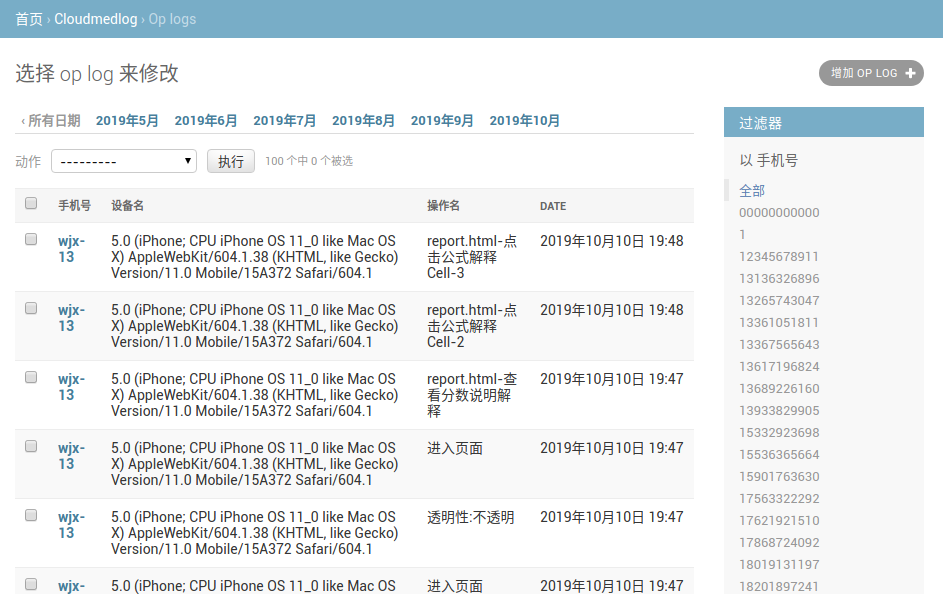
\includegraphics[width=12cm]{images/op_log.png}
    \caption{用户操作记录管理界面}
    \label{fig:op_log}
\end{figure}

\subsection{第三方问卷关联}
每次实验之前,根据实验的需求,可能需要先让用户填写一个问卷,收集必要的用户信息或者对用户进行评测;同样,在实验结束之后,也需要让用户填写问卷,收集用户反馈等。
在服务端重新实现问卷系统增加了工作量,本文通过接入第三方的问卷系统来实现,因此本系统需要对第三方的问卷系统提供对应的支持。


\begin{figure}[h]
    \centering
    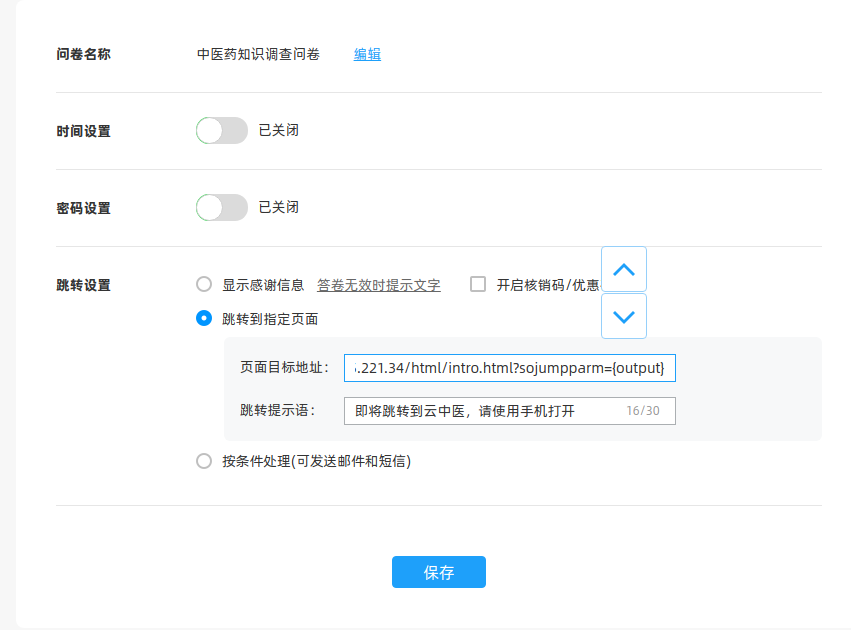
\includegraphics[width=10cm]{images/wjx1.png}
    \caption{第三方问卷系统跳转}
    \label{fig:wjx-ssojump}
\end{figure}

一次大致的实验流程为: 填写实验前问卷、进入面诊平台完成实验、填写反馈问卷。

在这个过程中,为了方便用户,本系统实现了第三方问卷支持,可以通过特定的地址参数完成从问卷到面诊平台完成自动登录。

如图\ref{fig:wjx-ssojump}所示,以问卷星为例,企业版的问卷星用户支持问卷完成后跳转到指定地址。指定的地址中可以带模板变量,如问卷的唯一id。
因此本文在系统登录页上只要判断是否存在该变量,如果存在则新建一个平台缩写+唯一id的用户名完成自动登录。


\subsection{任务处理}
一次用户诊断,服务端需要完成多个任务,目前支持的任务可以大致分类两类,计算任务和诊断任务。


\subsubsection{计算任务}
\begin{table}[]
    \centering
    \begin{tabular}{lll}
        \toprule
        字段 & 类型 & 描述 \\ 
        \midrule
        id & int & 主键 \\
        type & int & 任务类型: 面部,舌部,诊断,合并 \\ 
        extra & json & 模型相关信息 \\
        in & text & 任务输入 \\
        out & text & 任务结果 \\
        handler & text & 分配的服务端 \\
        status & int & 任务状态: 新建,已分配,处理中,失败,完成 \\
        createTime & datetime & 创建时间 \\
        updateTime & datetime & 更新时间\\
        \bottomrule
    \end{tabular}
    \caption{任务表}
    \label{tab:task}
\end{table}
计算任务对用户的输入进行计算,背后通过模型池中的模型来完成计算,如:面部特征提取任务,舌部特征提取任务,问诊任务。

服务端在收到用户提交的任务之后,会将数据存储到数据库的task表中,task表的主要字段如表 \ref{tab:task}所示:

\begin{enumerate}
    
    \item type一共有四种取值,目前对应四种任务类型:面部特征提取任务,舌部特征提取任务,诊断任务和合并任务。

    \item in为任务的输入,其中面部特征提取和舌部特征提取任务需要的输入为图片,通过Base64编码序列化为json对象,保存在in字段中。

    \item out为任务的执行结果,在模型池的服务完成计算之后,服务端将任务执行结果保存到out字段,同时更新任务的状态。

    \item  handler保存当前任务是由哪个服务端在负责处理。

    \item extra通过json格式存储模型相关信息,如分类任务,如体质判别,输出的7中体质的中文名称,保存在extra中。
\end{enumerate}

\subsubsection{诊断任务}
% 合并任务只有前置任务,没有后置任务,它是整个任务调度流程中的最后一个任务。合并任务的主要功能是在所有计算类型的任务完成后,对计算出来的结果进行合并。

% 合并任务的触发时机,是在合并任务的所有前置任务完成之后。合并任务的合并流程如下:

诊断任务的执行逻辑在服务端实现,不在模型池中有对应的模型。 诊断任务用于监测证整个图的顺利执行。

在各类任务完成之后,诊断任务通过从redis或者mysql中获取当前已完成任务的结果作为输入,完成最终的诊断。 
诊断任务的内部实现是有一套规则系统组成,定义了每一个任务的输入,会对最终的输出产生怎么样的影响。

在该模式下,本地系统可以比较方便的添加新的模型: 在一个新的模型添加到模型池之后,只需要在规则系统中,添加一条新的规则即可完成模型的接入。
这样,新模型可以通过规则系统中设置的规则,影响最终的结果。

\begin{figure}[ht]
    \centering
    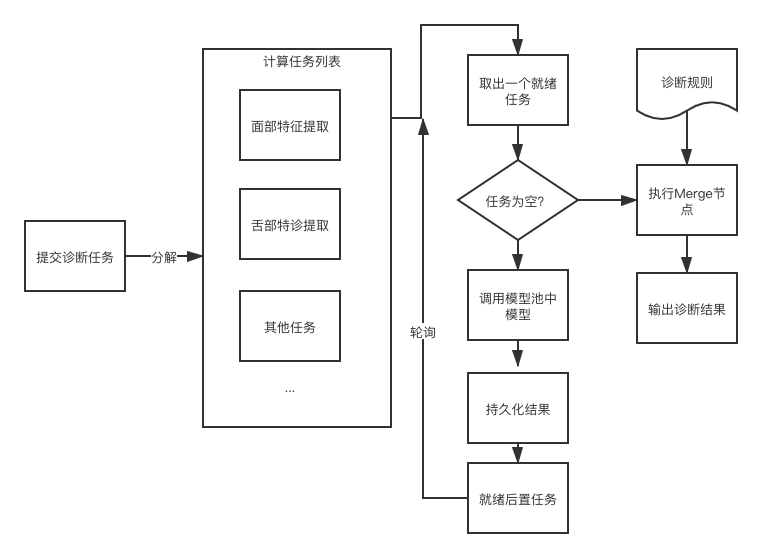
\includegraphics[width=12cm]{images/sketch2.png}
    \caption{诊断流程}
    \label{fig:sketch}
\end{figure}

诊断流程具体如图 \ref{fig:sketch} 所示:用户在提交诊断任务之后,服务端会将诊断任务分解成多个小的计算任务,其中包括面部特征提取,舌部特征提取以及其他相关的任务。任务分解的目的是降低单个服务端实例的计算压力,将任务计算分发到多个服务端,提高计算速度。
同时分解后的任务结果都保存在mysql数据库中,便于后续算法暴露中间结果给用户。
在任务分解之后,通过轮询选出其中一个未完成的任务,调用相关服务完成计算;如果计算任务事先已经完成计算,或者经过轮询已经完成所有的任务,则通过规则系统,取出计算任务的结果进行诊断。



\subsection{任务分配}
%为什么要这样做?
为了实现服务的稳定性,服务端支持同时开启多个实例,即多个服务端同时处理任务。
同时考虑到性能,服务端设计为读写分离的架构:每个实例都可以读取任务列表,处理用户的任务,但只有主节点有任务分配的权限。


\subsubsection{主从节点}
% 为什么要这样做
为了屏蔽用户间的设备差异,让硬件较差的用户设备也能调用模型,本系统采用算法模型和客户端剥离的方案。
模型和客户端剥离则增加了服务端的计算压力,对系统稳定性要求更高。
虽然目前已有大量成熟的服务发现、服务注册相关的框架,但为了使服务尽量轻量化,避免引入更多的依赖,简单的主从机制已经可以满足需要。
因此服务端通过实现简单的读写分离和主从竞选的机制,使得服务端支持同时运行多个实例,提高稳定性和性能。


大批量的用户请求需要服务的高可用。为了实现服务端的高可用,本文将服务端设计成允许多个实例同时运行。同时,如果不做主从节点划分,每次有可用的任务时,所有节点都去抢占任务,会有大量锁的竞争的问题。
因此本文将每个实例的角色划分为主节点和从节点进行读写分离,不同节点的具体职责如下:

\begin{enumerate}
    \item 主节点: 通过任务的id进行哈希,按照哈希进行任务的分配给各个节点,更新task表。分配任务时,只有主节点才有对任务表进行写操作的权限。

    \item 从节点: 每个从节点每过一定的间隔时间,就会去读取任务列表,开始执行任务列表里属于自己的任务。  

\end{enumerate}

基于此机制,服务的实现任务分配只由主节点去更新task表,而执行任务时每个节点只会执行分配给自己的任务。

\subsubsection{角色竞选流程}

\begin{figure}
    \centering
    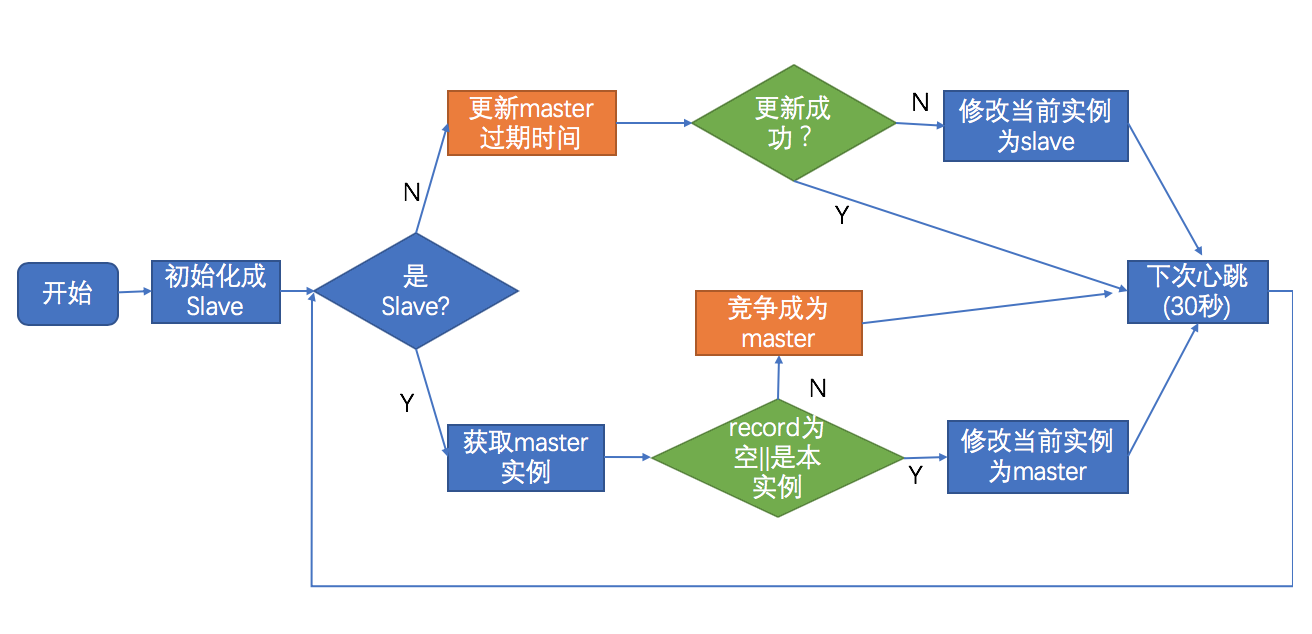
\includegraphics[width=10cm]{images/slave-master.png}
    \caption{服务端角色竞选}
    \label{fig:slave_master}
\end{figure}

服务端通过主从节角色分配的方式,同时运行多个实例来提高系统的响应速度,但多个实例同时运行也带来了系统稳定性的问题,如节点因为网络问题或者其他问题失效时,则需要通过心跳包探测节点存活。

服务端通过心跳包探活,主节点失效时,通过redis的分布式锁实现主节点的竞选。

每个节点在启动之后,会在本地把自己的角色默认设置成从节点。
然后每过一段时间,判断自己节点的类型,主从节点分别执行以下的心跳策略竞选主节点:

\begin{enumerate}
    \item 主节点:主节点每次心跳的时候,更新redis中主节点的过期时间。如果更新成功,等待下一次心跳; 如果更新失败(更新失败可能是自己没有及时更新,导致redis里的主节点过期,主节点的身份被其他节点竞争到了),则把自己的节点类型设置成从节点。
    
    \item 从节点:从节点每次从redis里获取主节点的信息,如果主节点信息无效或者长时间没有心跳(默认设置为两轮心跳周期),则开始抢占竞选锁,尝试更新redis的信息让自己成为主节点;如果redis的主节点信息已经是本节点,说明上一轮抢占成功,将本节点的角色更新为主节点。 
\end{enumerate}


\section{本章小结}
本章介绍了面诊系统的具体实现以解决上一章发现的技术敏感性问题与系统交互问题,其中面诊系统被划分为模型池、服务端和客户端。同时为了获取数据,服务端还提供了用户操作记录管理和问卷关联的功能,方便采集用户信息和后续分析用户行为。
在面诊系统的基础上,本文实现了两个交互设计,后续将在实验中验证本文所提出的设计策略的有效性。